\NeedsTeXFormat{LaTeX2e}
\documentclass[10pt,a4]{scrartcl}

\usepackage{tabularx,graphicx,a4}

\ifx\pdfoutput\undefined
  % We're not running pdftex
  % european (better) fonts -- does not look good with pdflatex
  \usepackage[T1]{fontenc}
  \newcommand{\href}[2]{#2\\{\hspace*{5mm}\scriptsize <#1>}\\}
\else
  \pdfcompresslevel=9
  \def\pdfBorderAttrs{/Border [0 0 0] } % No border around Links
  \usepackage{hyperref}
\fi

\title{Equalizer Programming Guide}
\author{Stefan Eilemann\thanks{eile@eyescale.ch}\\[\medskipamount]
  % Eyescale Software Sarl
}
\date{
  \textbf{INCOMPLETE}\\[\medskipamount]
  Version 0.1, \today
}

\newcommand{\tm}{\texttrademark~}
\newcommand{\rc}{\raise 1ex\hbox{{\tiny\textregistered}}~}
\newcommand{\fig}[1]{Figure~\ref{#1}}

% suppress  single floating lines on top (widow) and bottom(club)
%  10000 is infinity
%  tradeoff: maybe underfull vboxes
\clubpenalty=10000
\widowpenalty=10000 

\begin{document}

\maketitle
\vfill

\thispagestyle{empty}
\begin{figure}[ht]
  \centering
  
\includegraphics[width=4cm]{logo.pdf}
%  {\small\htmladdnormallink{www.eyescale.ch}{http://www.eyescale.ch}}
\end{figure}
\vfill

%\abstract{
%  Equalizer is a project to develop software to simplify the creation of
%  scalable graphics applications and to improve the usability of
%  multipipe visualization systems.
%}

\vfill {\center\begin{tabularx}{\textwidth}{|l|l|X|}
    \hline
    \bf Version & \bf Date     & \bf Changes \\
    \hline
    0.1         & Aug 19, 2007 & outlined the basic concepts\\
    \hline \multicolumn{3}{c}{\small
      \htmladdnormallink{http://www.equalizergraphics.com/documents/Developer/ProgrammingGuide.pdf}
      {http://www.equalizergraphics.com/documents/ProgrammingGuide.pdf}}\\
  \end{tabularx}}

\clearpage
\tableofcontents
\thispagestyle{empty}

\clearpage
\pagenumbering{arabic}

\section{Introduction}

Equalizer provides a framework for the development of parallel OpenGL
applications. Equalizer-based applications can run a single
shared-memory system with multiple graphics cards (GPU's) or on a
distributed graphics cluster. This Programming Guide introduces the
programming interface using the \textsf{eqPly} example shipped with Equalizer.

Any questions related to Equalizer programming and this Programming
Guide should be directed to the \textsf{eq-dev} mailing
list\footnote{see
  \htmladdnormallink{http://www.equalizergraphics.com/lists.html}
  {http://www.equalizergraphics.com/lists.html}}.

\section{Getting Started}

\subsection{Compiling and running \textsf{eqPly}}

A prerequisite for this Programming Guide is a working \textsf{eqPly}
example. The Quickstart
Guide\footnote{\htmladdnormallink{http://www.equalizergraphics.com/documents/EqualizerGuide.html}{http://www.equalizergraphics.com/documents/EqualizerGuide.html}}
explains how to run it. \textsf{eqPly} can also be executed without a
server, which simplifies the development cycle. In this case it will be
configured to use one window.

\subsection{Equalizer Processes}

\subsubsection{The Server}

An Equalizer server is responsible for managing one visualization
system\footnote{a shared memory system or graphics cluster}. Currently
it is only useful for running one application at a time, but it will be
extended to support multiple applications concurrently and efficiently
on one system. The server controls and potentially launches the
application's rendering clients.

\subsubsection{The Application}

The application connects to a server, which chooses a configuration for
the application. It provides a render client, to be launched by the
server. The application reacts on events and controls the rendering.

\subsubsection{The Render Client}

The render client implements the rendering part of an application. It is
passive, and receives all its rendering tasks from the server. The tasks
are executed by calling the appropriate task methods (see
\ref{ssTaskMethods}).

The application might be a rendering client, in which case it can also
contribute to the rendering. It can choose not to implement any render
client-related code, in which case it is reduced to be the application's
'master' process without any OpenGL windows.

The rendering client can be the same executable as the application, as
is the case with \textsf{eqPly}. Real-world applications often implement
a separate, light-weight rendering client.

\section{The Programming Interface}

Equalizer uses a C++ programming interface. The API is minimally
invasive, that is, Equalizer imposes only the minimal, natural execution
framework upon the application. It does not impose a scene graph or does
interfere in any way with the application's rendering code.

\subsection{\label{ssTaskMethods}Task Methods}

The application subclasses Equalizer objects and overrides virtual
functions to implement certain functionality, e.g., the OpenGL rendering
code in \textsf{eq::Channel::frameDraw}. These task methods are in
concept similar to C function callbacks.

\section{The Resource Tree}

The rendering resources are represented in a hierarchical tree structure
which corresponds to the physical and logical resources found in a 3D
rendering environment. 

\begin{figure}[ht]
  \centering
  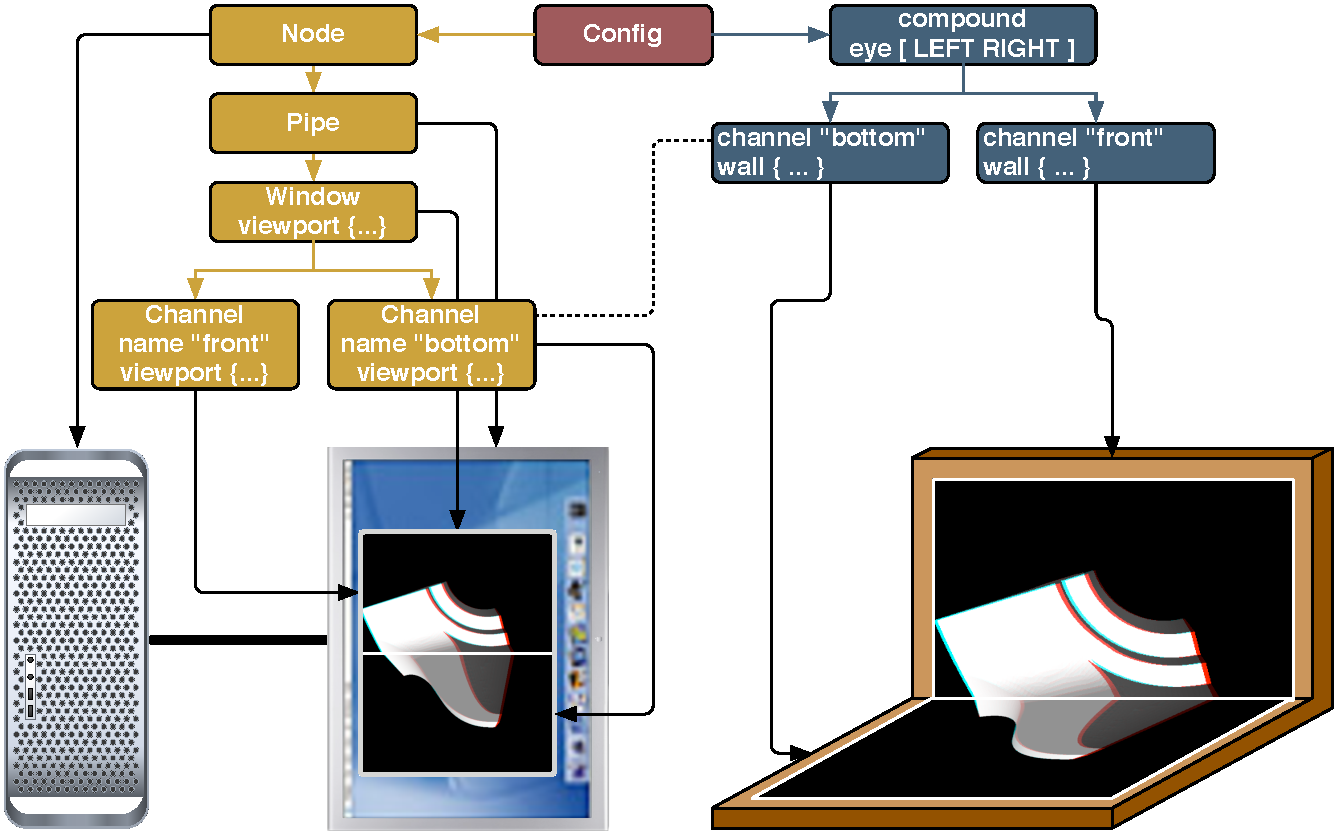
\includegraphics[width=\columnwidth]{desk.pdf}{\caption{\label{fConfig}An
      example configuration}}
\end{figure}

\fig{fConfig} shows one example configuration, running on a single
machine (node) using one graphics card (pipe) with one window to render
to two output channels connected to a L-shaped projection table. The
compound description is only used by the server to compute the rendering
tasks. The application is not aware of compounds, and does not need to
concern itself with the parallel rendering logics of a configuration.

For testing and development purposes it is possible to use multiple
instances for one resource, e.g., to run multiple render client nodes on
one computer. For deployment one node and pipe should be used for each
computer and graphics card, respectively.

\subsection{Configuration}

The root of the resource tree is the \textsf{eq::Config}, which
represents the current configuration of the application. It currently
only holds the local node, not all nodes of the configuration.

\subsection{Node}

An \textsf{eq::Node} is the representation of a single computer in the
system. It is one operating system process of the render client. All
node task methods are executed from the main application thread.

\subsection{Pipe}

The \textsf{eq::Pipe} is the abstraction of a graphics card (GPU). In
the current implementation it is also one operating system thread,
unless the pipe's thread hint is set to \textsf{false}. All pipe and
child window and channel task methods are executed from the pipe thread
for threaded pipes or from the main application thread for non-threaded
pipes\footnote{see also
  \htmladdnormallink{http://www.equalizergraphics.com/documents/design/nonthreaded.html}{http://www.equalizergraphics.com/documents/design/nonthreaded.html}
  for non-threaded rendering}.

Further versions of Equalizer might introduce threaded windows, where
all window-related task methods are executed in a separate operating
system thread.

\subsection{Window}

An \textsf{eq::Window} is an drawable and OpenGL context. The drawable
can be an on-screen window or an off-screen PBuffer or
FBO\footnote{off-screen drawables are not yet implemented, but can be
  created by the application and used with Equalizer}. 

\subsection{Channel}

The \textsf{eq::Channel} is the abstraction of an OpenGL viewport within
its parent window. It is the entity executing the actual rendering.

\bibliographystyle{abbrvurl}
\bibliography{paper}
\end{document}
